\subsection{Summary of Completed Research}

As with our content-driven reputation (described in Section~\ref{sec-reputation}),
our trust system analyzes the revision history of all wiki articles,
in chronological order.
The system assigns newly-inserted words an initial value of
trust proportional to the reputation of their author.
When subsequent authors edit the page, and leave the text surrounding
a word unchanged,  we raise the trust of the word.
On the other hand, if subsequent authors modify or rearrange the text
in proximity to the word, the trust in the word will, in general, decrease.
%
Specifically, when an author of reputation $r$
(generated from any reputation system, not necessarily
our content-driven reputation system) performs an edit
$\revision{k} : \version{k-1} \goesto \version{k}$,
we compute the maximal blocks of text that are
moved, inserted, or deleted during the edit.
We then compute the trust of the words in $\version{k}$ as follows
(see Figure~\ref{fig-trust-update} for a graphical representation):
%
\begin{itemize}

\item Newly-inserted words have a starting reputation that is equal to
  $\trustinherit \cdot r$, where $0 \le \trustinherit < 1$.

\item When a block of text is moved, the edges of the block represent
  discontinuities in the old content, and inherit trust
  $\trustinherit \cdot r$;
  this {\em edge effect\/} gradually fades towards the interior of the
  block, whose trust value is unchanged.
  This has the effect of highlighting areas near all forms of changes
  (because even insertions and deletions trigger move blocks in
  nearby text), drawing attention to the portions of text most
  likely to have changed in meaning.

\item When a block of text is deleted, it is preserved as ``dead
  text'' associated with the article, in case it is later
  re-inserted.
  The trust value of the text in the deleted block is lowered by an
  amount proportional to $r$, which prevents low reputation accounts
  from significantly altering the trust of text.
  Later insertions are compared against this dead text,
  which allows the original trust to be restored with the text
  if the deletion is reverted.

\item Once the above insertion, move, and deletion effects have taken
  place, we want to model author attention and give a little
  boost to words that the author has likely looked at.
  Given words that are in the same paragraph as a change
  that was made by the author,
  if the author reputation $r$ is greater than the trust $t$ of
  a word, the word trust is increased by the value
  $\partrust \cdot (r - t)$,
  where $0 \le \partrust < 1$.

\end{itemize}
%
A virtue of the system is that it makes it hard to maliciously
and surreptitiously change the content of Wikipedia articles: every
change, including text deletions, leaves a low-trust mark that fades
in future revisions only as the text is further revised.
Another property of our trust algorithm is that nobody can
single-handedly create fully trusted text: full trust (signaled via a
white background) can only be achieved via the edits of multiple
authors.
Finally, our treatment of deletions ensures that vandals cannot
reset the accumulated trust of the text in a page simply by deleting
it all: once the text is reinstated, it will have the same value of
trust it had immediately prior to deletion.


\begin{figure}[t]
\centering
\framebox{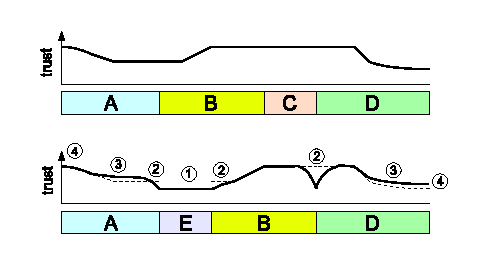
\includegraphics[width=0.55\textwidth]{part-F30-trust/trustalgo}}
\caption{Update process for text trust.
  The text is shown before (top) and after (bottom) an edit, together
  with its trust.
  In the bottom figure, the new values of trust (continuous line) are
  obtained from the inherited values of trust (dashed line) as follows:
  1: Trust value for newly inserted text (E).
  2: Edge effect: the text at the edge of blocks has the same trust as
  newly inserted text.
  3: Revision effect: old text may increase in trust, if the author
  reputation is higher than the old text trust.
  4: The edge effect is applied at the beginning and end of the
  article only if text changes there (which is not the case here).}
\label{fig-trust-update}
\end{figure}


To determine the parameters, we settled on the idea that
visualizing the trust should provide useful information
without innundating the user to the point of ignoring
the data.
That is, if all text is marked as untrustworthy,
then users will come to disregard the metric,
so we would prefer that pages be as ``white'' as possible.
To measure this, we defined the ``90\% white point'' of an
article as the 90\%-median
of the sorted trust values for each word in the article
(across all versions).
To capture the notion that low-trust reports meaningful
information, we also defined the ``weighted orange average''
to measure the average trust value of words which were
deleted in the next revision.
An important point is that vandals might erase perfectly good
text, which we are \textit{not} trying to flag with low trust;
we decide which deletions are relevant to us by referring back
to edit longevity.
Specifically, \elong is -1 when an edit is judged bad (as happens
when a vandal deletes text), and \elong is 1 when the edit is good.
We thus weight the trust of deleted words by the term
$\frac{\elong(\revision{k} + 1)}{2}$,
which has the effect of weighting by zero deletions done by vandals.
We combine these two measures into a single goal for optimization
by using the \intro{weighted harmonic mean}: $2 x y / (x+y)$
More details about the optimization can be found
in~\cite{WikiTrust2008}.


We have implemented the proposed system, and we have used it to color,
according to trust, the entire English Wikipedia, as of its February
6, 2007, snapshot (the most recent complete snapshot available);
the results can be viewed at \url{http://trust.cse.ucsc.edu}.

\subsubsection*{Quantitative Evaluation.}

How to evaluate the quality of our trust labeling was
a difficult question.
Our intuitive notion of trust was that it represents
the truthfulness of the text; this suggests that a manual
evaluation might be the most appropriate metric.
Such an approach would be very time consuming, however, and would
quickly discover that ``truth'' isn't something easily agreed upon.
Instead, we assess the quality of the trust labeling in a
data-driven way, using the idea that
trust should be a predictor for text stability~\cite{McGuinness06}.
% If low-trust is correlated with imprecise information, then low-trust
% text should be more likely to be subject to edits than high-trust
% text, as visitors and editors seek to correct the information.

We trained the coefficients involved in the computation of trust to be a
compromise between two goals: (a)~text, on average, is as
highly trusted as possible, and (b)~text that is going to deleted in
the next revision should be as low trust as possible.
After the training, we measured the quality of the trust coloring in
the following ways:
%
\begin{itemize}

\item {\em Recall of deletions.}
%  We consider the recall of low-trust as a predictor for deletions.
  We show that text in the lowest 50\% of trust values constitutes
  only 3.4\% of the text of articles, yet corresponds to 66\% of the
  text that is deleted from one revision to the next.

\item {\em Precision of deletions.}
%  We consider the precision of low-trust as a predictor for deletions.
  We show that text that is in the lowest 50\% of trust values has a
  probability of 33\% of being deleted in the very next revision, in
  contrast with the 1.9\% probability for general text.
  The deletion probability raises to 62\% for text in the bottom 20\%
  of trust values.

% \item {\em Trust of average vs. deleted text.}
%   We consider the trust distribution of all text, compared to the
%   trust distribution to the text that is deleted.
%   We show that 90\% of the text overall had trust at least 76\%, while
%   the average trust for deleted text was 33\%.

\item {\em Trust as a predictor of lifespan.}
%   We select words uniformly at random, and we consider the statistical
%   correlation between the trust of the word at the moment of
%   sampling, and the future lifespan of the word.
  We show that words with the highest trust have an expected future
  lifespan that is 4.5~times longer than words with no trust.

\end{itemize}
%
%
The above results were obtained by analyzing 1,000 articles selected
randomly from the Wikipedia articles with at least 200 revisions.
The requirement on the revision history ensures that each article has
a lifespan that is sufficiently long to analyze the predictive power
of trust with respect to text stability.
% We considered all text of all versions of the articles: overall, the
% selected articles contained 544,250 revisions, for a total of 13.74~GB
% of text.
% Taken together, these results indicate that the trust labeling we
% compute is a good predictor of future text stability.


